\documentclass[aspectratio=169, 11pt]{beamer}

% ── Theme & Colors (matched from enzyme_agent_workflow.tex) ──
\usetheme{Madrid}
\usecolortheme{default}

\definecolor{deepblue}{RGB}{20, 66, 114}
\definecolor{accentblue}{RGB}{41, 128, 185}
\definecolor{lightblue}{RGB}{214, 234, 248}
\definecolor{accentorange}{RGB}{230, 126, 34}
\definecolor{accentgreen}{RGB}{39, 174, 96}
\definecolor{darkgray}{RGB}{52, 73, 94}
\definecolor{lightgray}{RGB}{236, 240, 241}
\definecolor{accentred}{RGB}{192, 57, 43}
\definecolor{softpurple}{RGB}{142, 68, 173}

\setbeamercolor{structure}{fg=deepblue}
\setbeamercolor{palette primary}{bg=deepblue, fg=white}
\setbeamercolor{palette secondary}{bg=accentblue, fg=white}
\setbeamercolor{palette tertiary}{bg=deepblue!80, fg=white}
\setbeamercolor{frametitle}{bg=deepblue, fg=white}
\setbeamercolor{title}{fg=white}
\setbeamercolor{subtitle}{fg=lightblue}
\setbeamercolor{block title}{bg=accentblue, fg=white}
\setbeamercolor{block body}{bg=lightblue!30}
\setbeamercolor{block title alerted}{bg=accentorange, fg=white}
\setbeamercolor{block body alerted}{bg=accentorange!10}
\setbeamercolor{block title example}{bg=accentgreen, fg=white}
\setbeamercolor{block body example}{bg=accentgreen!10}
\setbeamercolor{item}{fg=accentblue}

\setbeamertemplate{navigation symbols}{}
\setbeamertemplate{footline}{%
  \hfill\insertframenumber/\inserttotalframenumber\hspace*{4pt}\vspace{2pt}%
}

% ── Packages ────────────────────────────────────────────────
\usepackage{tikz}
\usetikzlibrary{shapes.geometric, arrows.meta, positioning, calc, fit, backgrounds, decorations.pathreplacing}
\usepackage{booktabs}
\usepackage{graphicx}
\usepackage{colortbl}
\usepackage{adjustbox}
\usepackage{multirow}

\graphicspath{
  {../experimental_feedback/}
  {../experimental_feedback/analysis_results/}
  {../experimental_feedback/figures/}
  {../enzyme_agent_0427/summary/}
}

\title{LLM-Driven Enzyme Discovery \& Structural Validation}
\subtitle{Autonomous Biocatalyst Identification for Non-Natural Amide Synthesis}
\author{R. Zhu}
\date{\today}

\begin{document}

% ════════════════════════════════════════════════════════════
% SLIDE 1: Title
% ════════════════════════════════════════════════════════════
{
\setbeamercolor{background canvas}{bg=deepblue}
\begin{frame}[plain]
\vfill
\begin{center}
{\Huge\bfseries\color{white} Enzyme Discovery \& Structural Validation}\\[10pt]
{\Large\color{lightblue} An LLM-Driven Pipeline for\\Non-Natural Amide Bond Catalysis}\\[24pt]
{\large\color{white} R. Zhu}\\[6pt]
{\normalsize\color{lightblue!70} Group Meeting --- \today}
\end{center}
\vfill
\end{frame}
}

% ════════════════════════════════════════════════════════════
% SLIDE 2: Motivation
% ════════════════════════════════════════════════════════════
\begin{frame}{Motivation: Finding Enzymes for Nylon-6,6 Synthesis}
\begin{columns}[T]
\begin{column}{0.48\textwidth}
\begin{alertblock}{The Challenge}
\begin{itemize}
\item Target: enzymatic amide bond formation between \textbf{adipic acid} and \textbf{hexamethylenediamine} (nylon-6,6 monomers)
\item Relevant enzymes scattered across \textbf{6+ EC classes} and \textbf{diverse folds}
\item Manual search covers 2--3 obvious pathways; misses niche families
\item Need \textbf{biochemical reasoning}, not just keyword matching
\end{itemize}
\end{alertblock}
\end{column}
\begin{column}{0.48\textwidth}
\begin{exampleblock}{Two-Stage Approach}
\begin{enumerate}
\item \textbf{Discovery Agent}: autonomous LLM-driven search across databases and literature
\item \textbf{Structural Validation}: Boltz-2 co-folding to predict substrate binding and pocket compatibility
\end{enumerate}
\end{exampleblock}

\vspace{4pt}
\colorbox{lightblue!50}{\parbox{0.92\textwidth}{\centering
\small\textbf{Goal:} Go from target reaction to structurally validated candidates, ready for experimental testing.
}}
\end{column}
\end{columns}
\end{frame}

% ════════════════════════════════════════════════════════════
%  PART 1: ENZYME DISCOVERY AGENT
% ════════════════════════════════════════════════════════════
{
\setbeamercolor{background canvas}{bg=accentblue!90!black}
\begin{frame}[plain]
\vfill
\begin{center}
{\Large\bfseries\color{white} Part 1: Enzyme Discovery Agent}\\[10pt]
{\normalsize\color{lightblue!80} Autonomous search, evaluation, and ranking}
\end{center}
\vfill
\end{frame}
}

% ════════════════════════════════════════════════════════════
% SLIDE 3: System Architecture
% ════════════════════════════════════════════════════════════
\begin{frame}{System Architecture}
\vspace{-8pt}
\begin{columns}[T]
\begin{column}{0.40\textwidth}
\begin{center}
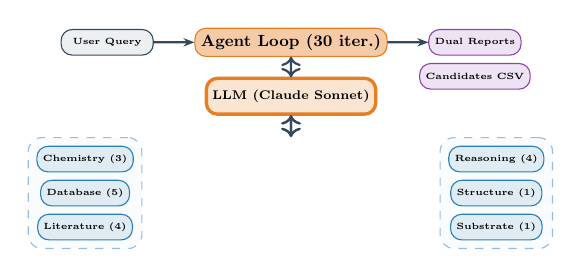
\begin{tikzpicture}[
    scale=0.65, transform shape,
    node distance=0.35cm,
    every node/.style={font=\small},
    box/.style={rectangle, rounded corners=4pt, minimum width=1.8cm, minimum height=0.5cm, text centered, font=\scriptsize\bfseries},
    llmbox/.style={box, fill=accentorange!20, draw=accentorange, line width=1.2pt, minimum width=2.8cm, minimum height=0.7cm},
    toolbox/.style={box, fill=accentblue!15, draw=accentblue, minimum width=1.6cm},
    outbox/.style={box, fill=softpurple!15, draw=softpurple, minimum width=1.8cm},
    arr/.style={-{Stealth[length=4pt]}, thick, color=darkgray},
]

% LLM Core
\node[llmbox] (llm) {LLM (Claude Sonnet)};

% Tool categories (left)
\node[toolbox, below left=0.6cm and 1.4cm of llm] (chem) {\tiny Chemistry (3)};
\node[toolbox, below=0.15cm of chem] (db) {\tiny Database (5)};
\node[toolbox, below=0.15cm of db] (lit) {\tiny Literature (4)};

% Tool categories (right)
\node[toolbox, below right=0.6cm and 1.4cm of llm] (reason) {\tiny Reasoning (4)};
\node[toolbox, below=0.15cm of reason] (struct) {\tiny Structure (1)};
\node[toolbox, below=0.15cm of struct] (sub) {\tiny Substrate (1)};

% Agent Loop
\node[box, fill=accentorange!40, draw=accentorange, above=0.4cm of llm, minimum width=3.5cm] (agent) {\small Agent Loop (30 iter.)};

% Input
\node[box, fill=lightgray, draw=darkgray, left=0.8cm of agent, minimum width=1.8cm, font=\tiny\bfseries] (input) {User Query};

% Outputs
\node[outbox, right=0.8cm of agent, font=\tiny\bfseries] (report) {Dual Reports};
\node[outbox, below=0.15cm of report, font=\tiny\bfseries] (csv) {Candidates CSV};

% Tool group fit
\begin{scope}[on background layer]
\node[fit=(chem)(db)(lit), draw=accentblue!50, dashed, rounded corners=5pt, inner sep=3pt, fill=accentblue!3] (leftfit) {};
\node[fit=(reason)(struct)(sub), draw=accentblue!50, dashed, rounded corners=5pt, inner sep=3pt, fill=accentblue!3] (rightfit) {};
\end{scope}

% Arrows
\draw[arr] (input) -- (agent);
\draw[arr] (agent) -- (report);
\draw[arr, <->] (agent) -- (llm);
\draw[arr, <->] (llm) -- (leftfit.north-|llm);
\draw[arr, <->] (llm) -- (rightfit.north-|llm);

\end{tikzpicture}
\end{center}
\end{column}

\begin{column}{0.57\textwidth}

\begin{block}{\small 18 Tools Across 6 Categories}
\vspace{-2pt}
\begin{itemize}\scriptsize
\setlength\itemsep{0pt}
\item[\tiny$\triangleright$] \textbf{Chemistry (3)}: SMILES validation, molecular properties, fingerprint similarity
\item[\tiny$\boxdot$] \textbf{Database (5)}: UniProt search/fetch, KEGG enzyme, InterPro, protein domains
\item[\tiny$\triangleleft$] \textbf{Literature (4)}: PubMed, OpenAlex, entity extraction, deep citation search
\item[\tiny$\star$] \textbf{Reasoning (4)}: notebook, screening, multi-source evaluation
\item[\tiny$\square$] \textbf{Structure (1)}: load PDB/AlphaFold
\quad \tiny$\circ$ \scriptsize\textbf{Substrate (1)}: 3D volume, functional groups
\end{itemize}
\vspace{-2pt}
\end{block}

\begin{exampleblock}{\small Key Design Choices}
\vspace{-2pt}
\begin{itemize}\scriptsize
\setlength\itemsep{0pt}
\item \textbf{No composite scoring}: raw data returned; LLM applies biochemical judgment
\item \textbf{Principle-driven}: 7 principles guide behavior; agent infers its own phase
\item \textbf{Reflection} every 5 iterations; search deduplication (Jaccard $\geq$0.90)
\item \texttt{@tool} decorator auto-generates schemas; 14/18 tools are parallel-safe
\end{itemize}
\vspace{-2pt}
\end{exampleblock}

\end{column}
\end{columns}
\end{frame}

% ════════════════════════════════════════════════════════════
% SLIDE 4: Phase 1 --- Reaction Analysis
% ════════════════════════════════════════════════════════════
\begin{frame}{Phase 1: Reaction Analysis --- The Coverage Engine}
\vspace{-6pt}
\begin{center}
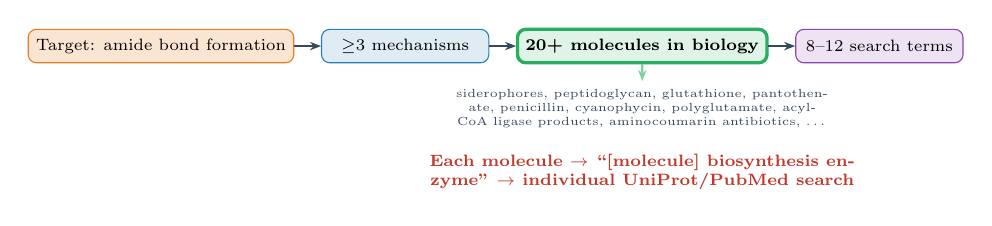
\begin{tikzpicture}[
    scale=0.85, transform shape,
    node distance=0.3cm,
    box/.style={rectangle, rounded corners=3pt, minimum height=0.5cm, text centered, font=\scriptsize, draw},
    arr/.style={-{Stealth[length=4pt]}, thick, color=darkgray},
]

\node[box, fill=accentorange!20, draw=accentorange, minimum width=2.8cm] (target) {Target: amide bond formation};
\node[box, fill=accentblue!15, draw=accentblue, right=0.4cm of target, minimum width=2.5cm] (mech) {$\geq$3 mechanisms};
\node[box, fill=accentgreen!15, draw=accentgreen, right=0.4cm of mech, minimum width=3.0cm, line width=1.2pt] (mol) {\textbf{20+ molecules in biology}};
\node[box, fill=softpurple!15, draw=softpurple, right=0.4cm of mol, minimum width=2.5cm] (search) {8--12 search terms};

\draw[arr] (target) -- (mech);
\draw[arr] (mech) -- (mol);
\draw[arr] (mol) -- (search);

\node[font=\tiny\color{darkgray}, below=0.25cm of mol, text width=7cm, align=center] (examples) {
siderophores, peptidoglycan, glutathione, pantothenate, penicillin, cyanophycin, polyglutamate, acyl-CoA ligase products, aminocoumarin antibiotics, \ldots
};

\draw[arr, dashed, color=accentgreen!60] (mol.south) -- (examples.north);

\node[font=\scriptsize\color{accentred}\bfseries, below=0.15cm of examples, text width=9cm, align=center] {
Each molecule $\rightarrow$ ``[molecule] biosynthesis enzyme'' $\rightarrow$ individual UniProt/PubMed search
};

\end{tikzpicture}
\end{center}

\vspace{-4pt}
\begin{columns}[T]
\begin{column}{0.48\textwidth}
\begin{block}{\small Steps A--D}
\begin{itemize}\scriptsize
\setlength\itemsep{1pt}
\item \textbf{A.} Classify bond type + reaction direction; identify substrate analogues
\item \textbf{B.} Enumerate $\geq$3 distinct mechanisms with different folds (e.g., NIS synthetase, ANL adenylation, Gln synthetase fold)
\item \textbf{C.} List 20+ molecules containing the bond across \textbf{8 biological contexts} (primary metabolism, cell wall, secondary metabolites, biopolymers, PTMs, xenobiotics, cofactors, signaling)
\item \textbf{D.} Write search specification \textit{before} any search tool call
\end{itemize}
\end{block}
\end{column}
\begin{column}{0.48\textwidth}
\begin{exampleblock}{\small Why This Drives Coverage}
\begin{itemize}\scriptsize
\setlength\itemsep{1pt}
\item \textbf{Bond-type search is exhaustive}: every biological context where the target bond occurs is enumerated
\item Manual search covers 2--3 obvious pathways; agent covers \textbf{all 8 contexts}
\item Each molecule becomes a \textit{specific} search term, avoiding the ``long query returns 0 results'' trap
\item Recorded in notebook section \texttt{enzyme\_landscape} for gap-checking in later phases
\end{itemize}
\end{exampleblock}
\end{column}
\end{columns}
\end{frame}

% ════════════════════════════════════════════════════════════
% SLIDE 5: Phase 2 --- Discovery
% ════════════════════════════════════════════════════════════
\begin{frame}{Phase 2: Multi-Axis Discovery}
\vspace{-6pt}
\begin{columns}[T]
\begin{column}{0.48\textwidth}

\begin{block}{\small Search Strategy}
For each molecule from Phase 1, the agent searches across \textbf{5 axes}:
\begin{enumerate}\scriptsize
\setlength\itemsep{1pt}
\item \textbf{KEGG} by all EC prefixes (complete + partial)
\item \textbf{UniProt} by individual gene names
\item \textbf{InterPro} by domain family
\item \textbf{PubMed/OpenAlex} with short 3--5 word queries
\item \textbf{Citation mining}: follow reference chains from seed papers
\end{enumerate}
\end{block}

\vspace{2pt}
\begin{alertblock}{\small Search Deduplication}
\vspace{-2pt}
\begin{itemize}\scriptsize
\setlength\itemsep{1pt}
\item Before executing any query, check if semantically similar query already ran
\item Similarity = max(Jaccard\textsubscript{tokens}, SequenceMatcher\textsubscript{chars})
\item Threshold $\geq$0.90 $\rightarrow$ return cached result with guidance to try different strategy
\end{itemize}
\end{alertblock}

\end{column}
\begin{column}{0.48\textwidth}

\begin{center}
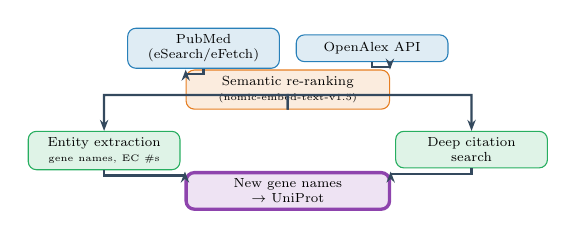
\begin{tikzpicture}[
    scale=0.68, transform shape,
    node distance=0.25cm,
    box/.style={rectangle, rounded corners=3pt, minimum height=0.5cm, text centered, font=\scriptsize, draw, text width=2.6cm},
    arr/.style={-{Stealth[length=4pt]}, thick, color=darkgray},
]

% Row 1: Search sources
\node[box, fill=accentblue!15, draw=accentblue] (pm) {PubMed\\(eSearch/eFetch)};
\node[box, fill=accentblue!15, draw=accentblue, right=0.3cm of pm] (oa) {OpenAlex API};

% Row 2: Semantic re-ranking
\node[box, fill=accentorange!15, draw=accentorange, below=0.4cm of $(pm)!0.5!(oa)$, minimum width=3.8cm] (rerank) {Semantic re-ranking\\{\tiny (nomic-embed-text-v1.5)}};

% Row 3: Entity extraction + Deep search
\node[box, fill=accentgreen!15, draw=accentgreen, below left=0.4cm and 0.1cm of rerank] (entity) {Entity extraction\\{\tiny gene names, EC \#s}};
\node[box, fill=accentgreen!15, draw=accentgreen, below right=0.4cm and 0.1cm of rerank] (deep) {Deep citation\\search};

% Row 4: New genes
\node[box, fill=softpurple!15, draw=softpurple, below=0.4cm of $(entity)!0.5!(deep)$, minimum width=3.8cm, line width=1.2pt] (genes) {New gene names $\rightarrow$ UniProt};

\draw[arr] (pm.south) -- ++(0,-0.1) -| (rerank.north west);
\draw[arr] (oa.south) -- ++(0,-0.1) -| (rerank.north east);
\draw[arr] (rerank) -- ++(0,-0.1) -| (entity.north);
\draw[arr] (rerank) -- ++(0,-0.1) -| (deep.north);
\draw[arr] (entity.south) -- ++(0,-0.1) -| (genes.north west);
\draw[arr] (deep.south) -- ++(0,-0.1) -| (genes.north east);

\end{tikzpicture}
\end{center}

\vspace{2pt}
\colorbox{lightblue!50}{\parbox{0.92\columnwidth}{\centering
\scriptsize \textbf{Citation mining}: abstracts lack gene names; \texttt{deep\_lit\_search} follows refs of top 3 papers $\rightarrow$ extracts names from \textit{their} titles. Discovers enzymes invisible to keyword search.
}}

\end{column}
\end{columns}
\end{frame}

% ════════════════════════════════════════════════════════════
% SLIDE 6: Phase 3 --- Candidate Evaluation
% ════════════════════════════════════════════════════════════
\begin{frame}{Phase 3: Candidate Evaluation}
\vspace{-6pt}
\begin{columns}[T]
\begin{column}{0.48\textwidth}

\begin{center}
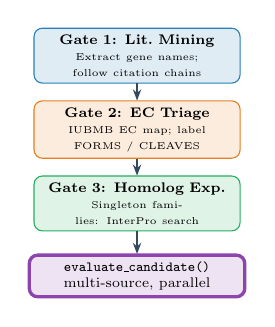
\begin{tikzpicture}[
    scale=0.72, transform shape,
    node distance=0.2cm,
    box/.style={rectangle, rounded corners=3pt, minimum height=0.5cm, text centered, font=\scriptsize, text width=3.4cm, draw},
    arr/.style={-{Stealth[length=4pt]}, thick, color=darkgray},
]

% Gate 1
\node[box, fill=accentblue!15, draw=accentblue] (g1) {\textbf{Gate 1: Lit.\ Mining}\\{\tiny Extract gene names; follow citation chains}};

% Gate 2
\node[box, fill=accentorange!15, draw=accentorange, below=0.3cm of g1] (g2) {\textbf{Gate 2: EC Triage}\\{\tiny IUBMB EC map; label FORMS / CLEAVES}};

% Gate 3
\node[box, fill=accentgreen!15, draw=accentgreen, below=0.3cm of g2] (g3) {\textbf{Gate 3: Homolog Exp.}\\{\tiny Singleton families: InterPro search}};

% Evaluate
\node[box, fill=softpurple!15, draw=softpurple, line width=1.2pt, below=0.4cm of g3, minimum width=3.8cm] (eval) {\textbf{\texttt{evaluate\_candidate()}}\\multi-source, parallel};

\draw[arr] (g1) -- (g2);
\draw[arr] (g2) -- (g3);
\draw[arr] (g3) -- (eval);

\end{tikzpicture}
\end{center}

{\centering\scriptsize\color{darkgray} All 3 gates trigger automatically when the LLM first calls \texttt{evaluate\_candidate}\par}

\end{column}
\begin{column}{0.48\textwidth}

\begin{alertblock}{\small Critical Warnings (Hard Gates)}
\vspace{-2pt}
\begin{itemize}\scriptsize
\setlength\itemsep{1pt}
\item \textbf{Bond-type mismatch}: enzyme cleaves amides but target is formation
\item \textbf{Reaction direction mismatch}: thermodynamically irreversible without cofactor change
\item \textbf{Severe size mismatch}: MW ratio $>$\,6.7$\times$
\end{itemize}
{\tiny\color{accentred} Cannot be overridden without specific PMID demonstrating target reaction}
\end{alertblock}

\vspace{2pt}
\begin{exampleblock}{\small Per-Substrate Scoring}
\vspace{-2pt}
\begin{itemize}\scriptsize
\setlength\itemsep{1pt}
\item Each target substrate scored independently
\item \textbf{Primary}: functional group counts (carboxyl, amine, hydroxyl, thiol)
\item \textbf{Secondary}: MW similarity, chain length, LogP
\item \textbf{Reference}: Tanimoto fingerprint (ECFP4)
\item Also gathers: UniProt annotations, PDB/AlphaFold structures, PubMed characterization \& engineering paper counts
\end{itemize}
\end{exampleblock}

\end{column}
\end{columns}
\end{frame}

% ════════════════════════════════════════════════════════════
% SLIDE 7: Phase 4 --- Ranking & Dual Reports
% ════════════════════════════════════════════════════════════
\begin{frame}{Phase 4: Ranking \& Dual Reports}
\vspace{-6pt}
\begin{columns}[T]
\begin{column}{0.48\textwidth}

\begin{block}{\small 4-Level Ranking Framework}
\vspace{-2pt}
\begin{itemize}\scriptsize
\setlength\itemsep{2pt}
\item[\textbf{P0.}] {\color{accentred}\textbf{Critical warnings}} $\rightarrow$ bottom tier (hard gate)
\item[\textbf{P1.}] \textbf{Substrate compatibility} (highest weight)\\
  {\tiny FG counts $>$ MW similarity $>$ Tanimoto}
\item[\textbf{P2.}] \textbf{Characterization depth}\\
  {\tiny Swiss-Prot curation, $\geq$5 kinetics/mechanism papers}
\item[\textbf{P3.}] \textbf{Structural data}\\
  {\tiny PDB $>$ AlphaFold $>$ none}
\item[\textbf{P4.}] \textbf{Engineering precedent}\\
  {\tiny $\geq$2 directed evolution / rational design papers}
\end{itemize}
\end{block}

\vspace{2pt}
\colorbox{lightblue!50}{\parbox{0.92\textwidth}{\centering
\scriptsize\textbf{Key insight:} The evaluator provides \textit{structured facts} (bond types, FG counts, MW ratios). The LLM provides \textit{biochemical judgment} (which facts matter for this specific target).
}}

\end{column}
\begin{column}{0.48\textwidth}

\begin{block}{\small Confidence-Weighted Report}
\vspace{-2pt}
\begin{itemize}\scriptsize
\setlength\itemsep{1pt}
\item Experimental evidence drives ranking position
\item Swiss-Prot curation, crystal structures $\rightarrow$ higher rank
\item \textbf{Use case}: start with the most well-understood enzyme
\end{itemize}
\end{block}

\vspace{2pt}
\begin{alertblock}{\small Suitability-Focused (Explorative) Report}
\vspace{-2pt}
\begin{itemize}\scriptsize
\setlength\itemsep{1pt}
\item Biochemical suitability drives ranking position
\item Evidence $\rightarrow$ separate confidence column, does \textbf{not} affect rank
\item \textbf{Use case}: find the biochemically closest enzyme, even if under-studied
\end{itemize}
\end{alertblock}

\vspace{2pt}
\colorbox{accentgreen!15}{\parbox{0.92\textwidth}{\centering
\scriptsize\textbf{Why two reports?} Same data, different criteria $\rightarrow$ surfaces \textbf{different candidates}. Under-characterized enzymes with excellent substrate match appear only in the explorative report.
}}

\end{column}
\end{columns}
\end{frame}

% ════════════════════════════════════════════════════════════
% SLIDE 5: Discovery Results
% ════════════════════════════════════════════════════════════
\begin{frame}{Discovery Results: Amide Synthetases for Nylon-6,6}
\vspace{-10pt}
\begin{center}
\scriptsize\color{darkgray} \textit{Adipic acid + hexamethylenediamine $\rightarrow$ amide bond (ATP-dependent)}
\end{center}
\vspace{-2pt}

{\scriptsize
\begin{adjustbox}{max width=\textwidth}
\begin{tabular}{@{}c l l l l p{5.5cm}@{}}
\toprule
\textbf{Rank} & \textbf{Gene} & \textbf{Family} & \textbf{Organism} & \textbf{Evidence} & \textbf{Key Rationale}\\
\midrule
1 & \texttt{asbA} & NIS synthetase & \textit{B.\,anthracis} & Swiss-Prot &
Perfect FG match on spermidine amine; documented diamine + diacid promiscuity\\
2 & \texttt{asbB} & NIS synthetase & \textit{B.\,anthracis} & PDB 3TO3, 4 mut. &
K313A/M variants accept linear diamines (HMD-like); best engineering tractability\\
3 & \texttt{puuA} & Gln syn.\ fold & \textit{E.\,coli} K12 & 2 mut., 2 eng. &
Glutamate MW = adipate MW (146--147 Da); accepts cadaverine/spermidine\\
4 & \texttt{iucA} & NIS synthetase & \textit{E.\,coli} & 9 char.\ papers &
Well-characterized NIS; citrate acid substrate closest to adipic acid\\
5 & \texttt{iucC} & NIS synthetase & \textit{E.\,coli} & 19 char., 2 eng. &
Most-characterized NIS synthetase; standard reference enzyme\\
\bottomrule
\end{tabular}
\end{adjustbox}
}

\vspace{4pt}
\begin{columns}[T]
\begin{column}{0.32\textwidth}
\begin{block}{\scriptsize Scale}
\centering\scriptsize
\textbf{27 candidates} evaluated\\across \textbf{6 enzyme families}\\
18 iterations, 2.5M tokens
\end{block}
\end{column}
\begin{column}{0.32\textwidth}
\begin{exampleblock}{\scriptsize Key Finding}
\centering\scriptsize
NIS synthetases natively\\couple diacids to diamines\\via ATP --- same chemistry
\end{exampleblock}
\end{column}
\begin{column}{0.32\textwidth}
\begin{alertblock}{\scriptsize Question}
\centering\scriptsize
Good on paper, but does\\the substrate \textbf{physically fit}\\in the active site?
\end{alertblock}
\end{column}
\end{columns}
\end{frame}

% ════════════════════════════════════════════════════════════
%  PART 2: STRUCTURAL MODELING
% ════════════════════════════════════════════════════════════
{
\setbeamercolor{background canvas}{bg=accentblue!90!black}
\begin{frame}[plain]
\vfill
\begin{center}
{\Large\bfseries\color{white} Part 2: Structural Validation}\\[10pt]
{\normalsize\color{lightblue!80} Co-folding, pocket chemistry, and substrate compatibility}
\end{center}
\vfill
\end{frame}
}

% ════════════════════════════════════════════════════════════
% SLIDE 6: Why Structural Modeling?
% ════════════════════════════════════════════════════════════
\begin{frame}{Why Structural Modeling?}
\begin{columns}[T]
\begin{column}{0.48\textwidth}
\begin{alertblock}{The Problem}
\begin{itemize}
\item Discovery agent ranks by \textbf{sequence \& literature}
\item But: does the substrate \textbf{physically fit}?
\item Is the pocket \textbf{chemically compatible}?
\item Is the substrate \textbf{positioned for catalysis}?
\end{itemize}
\end{alertblock}
\vspace{4pt}
\colorbox{accentred!15}{\parbox{0.92\textwidth}{\centering\small
\textbf{McbA:} iPTM = 0.987, hydrophobicity = 42.9\%\\
\textit{yet experimentally inactive}
}}
\end{column}
\begin{column}{0.48\textwidth}
\begin{exampleblock}{Our Approach}
\begin{itemize}
\item \textbf{Co-fold} each candidate with substrates + cofactors using Boltz-2
\item Extract \textbf{binding geometry}, \textbf{pocket chemistry}, \textbf{pocket stability}
\item Compare \textbf{apo vs.\ holo} pockets
\item \textbf{122 complexes}: 29 synthetases + 93 hydrolases
\end{itemize}
\end{exampleblock}
\end{column}
\end{columns}

\vspace{4pt}
\begin{center}
\colorbox{lightblue!50}{\parbox{0.88\textwidth}{\centering
\small\textbf{Goal:} Structural evidence for \textit{which} candidates to test and \textit{why} others should be deprioritized.
}}
\end{center}
\end{frame}

% ════════════════════════════════════════════════════════════
% SLIDE 7: Co-folding Pipeline
% ════════════════════════════════════════════════════════════
\begin{frame}{Co-folding Pipeline Overview}
\vspace{-8pt}
\begin{center}
\includegraphics[height=0.62\textheight]{cofold_pipeline.png}
\end{center}
\vspace{-6pt}
\begin{columns}[T]
\begin{column}{0.32\textwidth}
\begin{block}{\scriptsize Cofactor-Guided (28 syn.)}
\vspace{-2pt}
\begin{itemize}\scriptsize
\setlength\itemsep{0pt}
\item ATP constrained to AlphaFill pocket
\item Substrates dock \textbf{freely} nearby
\item \textcolor{accentgreen}{Independent validation}
\end{itemize}
\end{block}
\end{column}
\begin{column}{0.32\textwidth}
\begin{alertblock}{\scriptsize Pocket-Constrained (89 hyd.)}
\vspace{-2pt}
\begin{itemize}\scriptsize
\setlength\itemsep{0pt}
\item Substrates anchored to predicted pocket
\item \textcolor{accentorange}{Circular with selection}
\end{itemize}
\end{alertblock}
\end{column}
\begin{column}{0.32\textwidth}
\begin{block}{\scriptsize Scoring (8 metrics)}
\vspace{-2pt}
\begin{itemize}\scriptsize
\setlength\itemsep{0pt}
\item iPTM, SASA burial
\item Pocket chemistry (\% hydro/charged/polar)
\item Steric clashes, volume ratio
\end{itemize}
\end{block}
\end{column}
\end{columns}
\end{frame}

% ════════════════════════════════════════════════════════════
% SLIDE 8: Pocket Chemistry Landscape
% ════════════════════════════════════════════════════════════
\begin{frame}{Pocket Chemistry: Synthetases vs.\ Hydrolases}
\vspace{-8pt}
\begin{columns}[T]
\begin{column}{0.52\textwidth}
\begin{center}
\includegraphics[width=\textwidth]{pocket_chemistry_landscape_backup.png}
\end{center}
\end{column}
\begin{column}{0.45\textwidth}
\vspace{6pt}
\begin{center}
\scriptsize
\begin{tabular}{lcc}
\toprule
\textbf{Pocket comp.} & \textbf{Syn.} & \textbf{Hyd.} \\
& {\tiny ($n$=29)} & {\tiny ($n$=93)} \\
\midrule
Hydrophobic & \textbf{34.3\%} & 30.5\% \\
{\tiny \textit{p} = 0.031} & & \\
Charged & 31.5\% & 29.2\% \\
{\tiny \textit{p} = 0.16 (n.s.)} & & \\
Polar & \textbf{34.2\%} & 40.3\% \\
{\tiny \textit{p} $<$ 0.001} & & \\
\midrule
\textbf{NylC ref.} & \multicolumn{2}{c}{\textbf{40.5\%} hydro, \textbf{8.1\%} charged} \\
\bottomrule
\end{tabular}
\end{center}

\vspace{6pt}
\begin{exampleblock}{\scriptsize Key Observation}
\vspace{-2pt}
\scriptsize
NylC ({\color{accentgreen}$\bigstar$}) is a clear outlier: 40\% hydrophobic, only 8\% charged. This pocket profile matches the 68\% aliphatic nylon backbone.
\end{exampleblock}
\end{column}
\end{columns}
\end{frame}

% ════════════════════════════════════════════════════════════
% SLIDE 9: Native Substrate Diversity
% ════════════════════════════════════════════════════════════
\begin{frame}{Native Substrate Diversity}
\vspace{-8pt}
\begin{columns}[T]
\begin{column}{0.52\textwidth}
\begin{center}
\includegraphics[width=0.95\textwidth,height=0.68\textheight,keepaspectratio]{substrate_diversity.png}
\end{center}
\end{column}
\begin{column}{0.45\textwidth}
\vspace{2pt}
\begin{block}{\small Why This Matters}
\begin{itemize}\scriptsize
\setlength\itemsep{0pt}
\item Native substrates reveal what each enzyme \textbf{evolved to bind}
\item Nylon monomers are \textbf{small, linear, aliphatic}: adipic acid (146 Da), HMD (116 Da)
\item Best candidates: native substrates with \textbf{similar size and chemistry}
\item PuuA: glutamate (147 Da) $\approx$ adipic acid (146 Da)
\item AsbA/B: spermidine (2 primary amines) $\approx$ HMD
\end{itemize}
\end{block}

\vspace{2pt}
\colorbox{lightblue!50}{\parbox{0.92\textwidth}{\centering
\scriptsize Substrate diversity analysis bridges sequence-level discovery with structural pocket compatibility.
}}
\end{column}
\end{columns}
\end{frame}

% ════════════════════════════════════════════════════════════
% SLIDE 10: Hydrolase Inactivity
% ════════════════════════════════════════════════════════════
\begin{frame}{Why 93 Screened Hydrolases Failed}
\vspace{-6pt}

\begin{columns}[T]
\begin{column}{0.48\textwidth}

\begin{center}
\scriptsize
\begin{tabular}{lccr}
\toprule
\textbf{Metric} & \textbf{Syn.} & \textbf{Hyd.} & \textbf{\textit{p}} \\
& {\tiny ($n$=29)} & {\tiny ($n$=93)} & \\
\midrule
iPTM & \textbf{0.913} & 0.748 & $<$0.001 \\
SASA burial & \textbf{86.1\%} & 61.5\% & $<$0.001 \\
Hydrophobic & \textbf{34.3\%} & 30.5\% & 0.031 \\
Polar & 34.2\% & \textbf{40.3\%} & $<$0.001 \\
\midrule
Pocket too small & 2 & \textcolor{accentred}{\textbf{41}} & --- \\
Groove binding & 0 & \textcolor{accentred}{\textbf{23}} & --- \\
\bottomrule
\end{tabular}
\end{center}

\vspace{4pt}
\colorbox{accentred!15}{\parbox{0.92\textwidth}{\centering\small
Nylon-6,6 trimer is \textbf{68\% aliphatic}\\(28 methylene groups, only 2 terminal charges)
}}

\end{column}
\begin{column}{0.48\textwidth}

\begin{alertblock}{\small Three Convergent Failures}
\begin{enumerate}\scriptsize
\setlength\itemsep{3pt}
\item \textbf{Pocket chemistry mismatch}: evolved for \textbf{charged} polymers (polyglutamate, cyanophycin), not aliphatic nylon; 29\% charged vs.\ NylC's 8\%
\item \textbf{Poor substrate accommodation}: 44\% pockets too small, 25\% groove-bound; cannot productively capture the large, flexible trimer (622 Da, 28 rotatable bonds)
\item \textbf{Catalytic mechanism}: isopeptidases cleave \textbf{branched side-chain} amides, not linear backbone amides
\end{enumerate}
\end{alertblock}

\vspace{2pt}
\colorbox{lightblue!50}{\parbox{0.92\textwidth}{\centering
\scriptsize The 93 hydrolases serve as a \textbf{structural negative control}: engineering NylC is more viable than repurposing isopeptidases.
}}

\end{column}
\end{columns}
\end{frame}

% ════════════════════════════════════════════════════════════
% SLIDE 11: Recommended Test Set
% ════════════════════════════════════════════════════════════
\begin{frame}{Recommended Experimental Test Set}
\vspace{-6pt}

\begin{center}
\begin{adjustbox}{max width=\textwidth}
\small
\begin{tabular}{clccccl}
\toprule
\textbf{\#} & \textbf{Gene} & \textbf{Sub.\ iPTM} & \textbf{SASA} & \textbf{Hydro.} & \textbf{Jaccard} & \textbf{Why this candidate?} \\
\midrule
1 & \textbf{PanC} & 0.914 & 97.8\% & \textbf{48.2\%} & \textbf{0.889} & Pantoate $\approx$ adipic acid; 100\% cat.\ center; \textit{E. coli} \\
2 & \textbf{GshA} & 0.959 & 82.4\% & 29.0\% & \textcolor{accentred}{0.025} & Glutamate (147 Da) $\approx$ adipic acid (146 Da); \textit{E. coli} \\
3 & \textbf{BacD} & 0.907 & 93.5\% & 40.7\% & \textbf{0.914} & Proven broad specificity; 8 mutagenesis variants \\
4 & \textbf{gss} & 0.936 & 95.3\% & 33.8\% & 0.812 & Phosphorylation mechanism (diversity); \textit{E. coli} \\
5 & \textbf{DdaF} & 0.963 & 78.6\% & 39.7\% & 0.829 & Highest sub.\ iPTM; follow-up candidate \\
\bottomrule
\end{tabular}
\end{adjustbox}
\end{center}

\vspace{4pt}
\begin{columns}[T]
\begin{column}{0.32\textwidth}
\begin{exampleblock}{\small Strongest Structural}
\centering\small
\textbf{PanC}: highest hydrophobicity, most stable pocket, 100\% catalytic overlap
\end{exampleblock}
\end{column}
\begin{column}{0.32\textwidth}
\begin{alertblock}{\small Strongest Chemical}
\centering\small
\textbf{GshA}: best MW match but low Jaccard --- tests if analogy alone predicts activity
\end{alertblock}
\end{column}
\begin{column}{0.32\textwidth}
\begin{block}{\small Best Engineered}
\centering\small
\textbf{BacD}: known mutations + most stable pocket (Jaccard = 0.914)
\end{block}
\end{column}
\end{columns}

\vspace{2pt}
\colorbox{lightgray}{\parbox{0.94\textwidth}{\centering\small
\textbf{Previously tested:} McbA (inactive --- geometry mismatch) + PylC (failed expression --- archaeal protein)
}}
\end{frame}

% ════════════════════════════════════════════════════════════
% SLIDE 12: Structural Renderings
% ════════════════════════════════════════════════════════════
\begin{frame}{Top Candidate Structures (Boltz-2 Co-folded)}
\vspace{-8pt}
\begin{columns}[c]
\begin{column}{0.48\textwidth}
\begin{center}
\includegraphics[width=0.92\textwidth]{struct_PanC_P31663_holo.png}\\[2pt]
{\small\textbf{PanC} (P31663) --- Rank \#1}\\
{\scriptsize\color{darkgray} Pocket hydrophobicity: 48.2\%, SASA: 97.8\%}
\end{center}
\end{column}
\begin{column}{0.48\textwidth}
\begin{center}
\includegraphics[width=0.92\textwidth]{struct_BacD_P39641_holo.png}\\[2pt]
{\small\textbf{BacD} (P39641) --- Rank \#3}\\
{\scriptsize\color{darkgray} Pocket hydrophobicity: 40.7\%, Jaccard: 0.914}
\end{center}
\end{column}
\end{columns}

\vspace{4pt}
\begin{center}
\colorbox{lightblue!50}{\parbox{0.80\textwidth}{\centering
\scriptsize Boltz-2 co-folding with ATP + Mg$^{2+}$ + substrates. Protein surface colored by hydrophobicity. Substrates shown as sticks.
}}
\end{center}
\end{frame}

% ════════════════════════════════════════════════════════════
%  PART 3: CLOSING
% ════════════════════════════════════════════════════════════

% ════════════════════════════════════════════════════════════
% SLIDE 13: End-to-End Pipeline
% ════════════════════════════════════════════════════════════
\begin{frame}{End-to-End: From Target Reaction to Experimental Candidates}
\vspace{-4pt}
\begin{center}
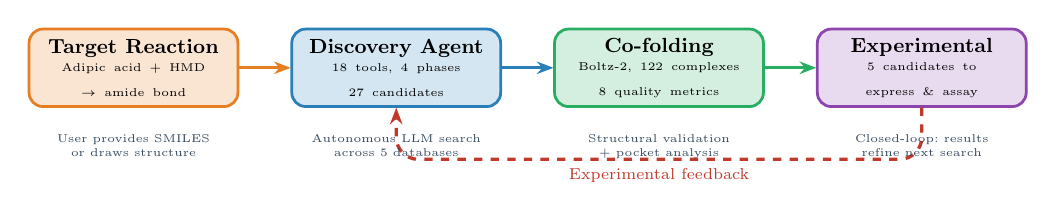
\begin{tikzpicture}[
    scale=0.82, transform shape,
    node distance=0.4cm,
    box/.style={rectangle, rounded corners=5pt, minimum height=1.2cm, text centered, font=\small\bfseries, text width=3.0cm, draw, line width=1pt},
    arr/.style={-{Stealth[length=6pt]}, very thick, color=darkgray},
    note/.style={font=\tiny\color{darkgray}, text width=3.0cm, align=center},
]

% Boxes
\node[box, fill=accentorange!20, draw=accentorange] (query) {
\small Target Reaction\\[2pt]
\tiny\normalfont Adipic acid + HMD\\$\rightarrow$ amide bond
};

\node[box, fill=accentblue!20, draw=accentblue, right=0.8cm of query] (agent) {
\small Discovery Agent\\[2pt]
\tiny\normalfont 18 tools, 4 phases\\27 candidates
};

\node[box, fill=accentgreen!20, draw=accentgreen, right=0.8cm of agent] (cofold) {
\small Co-folding\\[2pt]
\tiny\normalfont Boltz-2, 122 complexes\\8 quality metrics
};

\node[box, fill=softpurple!20, draw=softpurple, right=0.8cm of cofold] (test) {
\small Experimental\\[2pt]
\tiny\normalfont 5 candidates to\\express \& assay
};

% Arrows
\draw[arr, color=accentorange] (query) -- (agent);
\draw[arr, color=accentblue] (agent) -- (cofold);
\draw[arr, color=accentgreen] (cofold) -- (test);

% Feedback arrow
\draw[arr, color=accentred, dashed, rounded corners=8pt] (test.south) -- ++(0,-0.8) -| (agent.south) node[pos=0.25, below, font=\scriptsize\color{accentred}] {Experimental feedback};

% Annotations below
\node[note, below=0.3cm of query] {User provides SMILES\\or draws structure};
\node[note, below=0.3cm of agent] {Autonomous LLM search\\across 5 databases};
\node[note, below=0.3cm of cofold] {Structural validation\\+ pocket analysis};
\node[note, below=0.3cm of test] {Closed-loop:~results\\refine next search};

\end{tikzpicture}
\end{center}

\vspace{4pt}
\begin{columns}[T]
\begin{column}{0.48\textwidth}
\begin{block}{\small What the Agent Provides}
\begin{itemize}\scriptsize
\item Ranked candidate list with literature evidence
\item Native reaction comparison (FG counts, Tanimoto)
\item Dual reports (confidence vs.\ suitability)
\end{itemize}
\end{block}
\end{column}
\begin{column}{0.48\textwidth}
\begin{block}{\small What Co-folding Adds}
\begin{itemize}\scriptsize
\item Physical substrate fit (iPTM, SASA burial)
\item Pocket chemistry compatibility
\item Apo vs.\ holo pocket stability (Jaccard)
\item Negative control (93 hydrolases)
\end{itemize}
\end{block}
\end{column}
\end{columns}
\end{frame}

% ════════════════════════════════════════════════════════════
% SLIDE 14: Next Steps
% ════════════════════════════════════════════════════════════
\begin{frame}{Next Steps}
\vspace{-4pt}
\begin{columns}[T]
\begin{column}{0.48\textwidth}
\begin{block}{Experimental}
\begin{itemize}
\item Express \& assay \textbf{5 candidates} in \textit{E. coli}
\item Each tests a \textbf{structural hypothesis}:
  \begin{itemize}\small
  \item PanC: substrate similarity + pocket stability
  \item GshA: MW analogy vs.\ low Jaccard
  \item BacD: broad specificity + stable pocket
  \item gss: alternative activation mechanism
  \item DdaF: high iPTM, moderate chemistry
  \end{itemize}
\item Feed results back to discovery agent
\end{itemize}
\end{block}
\end{column}

\begin{column}{0.48\textwidth}
\begin{exampleblock}{Computational}
\begin{itemize}
\item \textbf{Catalytic geometry}: near-attack distances \& B\"urgi--Dunitz angles from co-folded structures
\item \textbf{Cross-family comparison}: how do NIS, ATP-grasp, and Mur ligase folds position the same substrates?
\item \textbf{McbA lesson}: binding $\neq$ catalysis; need spatially resolved descriptors beyond pocket composition
\end{itemize}
\end{exampleblock}
\end{column}
\end{columns}

\vspace{6pt}
\colorbox{accentgreen!15}{\parbox{0.88\textwidth}{\centering
\textbf{The question is not which candidates are active, but which structural hypotheses hold} --- revealing whether substrate similarity, pocket composition, or catalytic geometry best predicts activity on non-natural substrates.
}}
\end{frame}

% ════════════════════════════════════════════════════════════
% SLIDE 15: Summary
% ════════════════════════════════════════════════════════════
{
\setbeamercolor{background canvas}{bg=deepblue}
\begin{frame}[plain]
\vfill
\begin{center}
{\Large\bfseries\color{white} Summary}\\[16pt]
{\normalsize\color{lightblue}
\begin{tabular}{rl}
\color{accentorange}{18} & \color{white} specialized tools orchestrated by LLM agent \\[6pt]
\color{accentorange}{27+28} & \color{white} enzyme candidates discovered (synthetases + hydrolases) \\[6pt]
\color{accentorange}{122} & \color{white} enzyme--substrate complexes co-folded with Boltz-2 \\[6pt]
\color{accentorange}{93} & \color{white} hydrolases serve as structural negative control \\[6pt]
\color{accentorange}{5} & \color{white} candidates prioritized for experimental testing \\[6pt]
\color{accentorange}{1} & \color{white} key lesson: McbA shows that binding $\neq$ catalysis \\[6pt]
\end{tabular}
}
\end{center}
\vfill
\end{frame}
}

\end{document}
